% uPyCore memory system (main @ b90e881). Standalone TikZ figure sized for
% one ISCA column (3.33 in). Build: pdflatex memory_system.tex
% In the paper: \includegraphics[width=\columnwidth]{figures/memory_system.pdf}
\documentclass[tikz,border=1pt]{standalone}
\usepackage{newtxtext,newtxmath}
\usetikzlibrary{positioning,arrows.meta,calc,decorations.pathreplacing}
\begin{document}
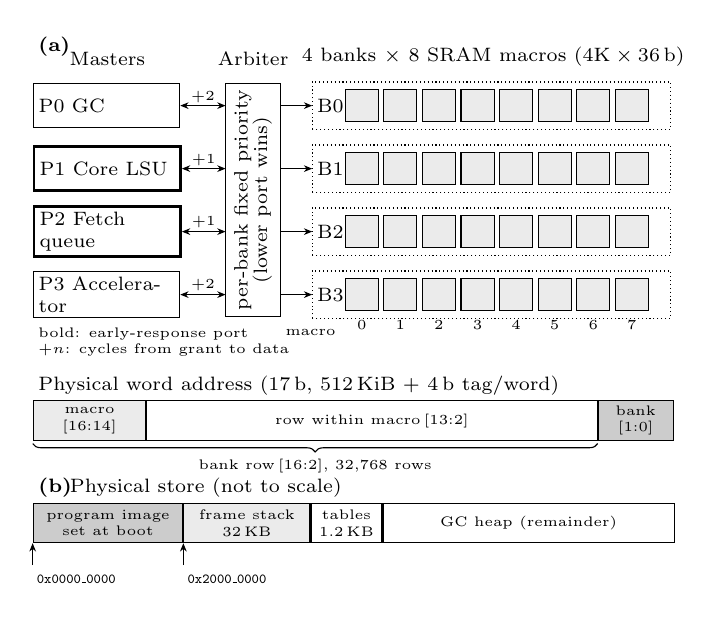
\begin{tikzpicture}[
  font=\scriptsize,
  >={Stealth[length=3pt,width=2.4pt]},
  port/.style={draw,thin,text width=1.72cm,minimum height=0.56cm,inner sep=2pt,align=left},
  early/.style={port,line width=1.0pt},
  mac/.style={draw,thin,fill=black!8,minimum width=0.42cm,minimum height=0.40cm,inner sep=0pt},
  bank/.style={draw,thin,densely dotted},
  fld/.style={draw,thin,minimum height=0.50cm,inner sep=0pt,font=\tiny,align=center},
]
% ---------------------------------------------------------------- (a)
\node[font=\scriptsize\bfseries,anchor=west] at (-0.05,3.75) {(a)};
\node[anchor=south] at (0.95,3.38) {Masters};
\node[anchor=south] at (2.80,3.38) {Arbiter};
\node[anchor=south] at (5.85,3.38) {4 banks $\times$ 8 SRAM macros ($4\mathrm{K}\times36$\,b)};

\foreach \i/\name/\lat/\sty in {0/GC/2/port,1/Core LSU/1/early,2/Fetch queue/1/early,3/Accelerator/2/port}{
  \pgfmathsetmacro{\y}{3.0-0.8*\i}
  \node[\sty,anchor=west] (p\i) at (0,\y) {P\i\ \name};
  \draw[<->] (p\i.east) -- node[above,font=\tiny,inner sep=1pt] {$+\lat$} (2.45,\y);
  % bank row
  \draw[bank] (3.55,\y-0.30) rectangle (8.10,\y+0.30);
  \node[anchor=west,inner sep=1pt] at (3.57,\y) {B\i};
  \foreach \m in {0,...,7}{
    \node[mac] (m\i\m) at (4.18+0.49*\m,\y) {};
  }
  \draw[->] (3.15,\y) -- (3.55,\y);
}
\draw[thin] (2.45,0.32) rectangle (3.15,3.28);
\node[rotate=90,align=center] at (2.80,1.80) {per-bank fixed priority\\[-1pt] (lower port wins)};
% macro index under the last bank
\foreach \m in {0,...,7}{\node[font=\tiny,below=0pt of m3\m] {\m};}
\node[font=\tiny,anchor=east] at (3.97,0.12) {macro};
\node[font=\tiny,anchor=west,align=left] at (-0.05,0.0) {bold: early-response port\\$+n$: cycles from grant to data};

% address bit field: 17 bits over 8.1 cm
\def\bw{0.4765}
\node[anchor=west] at (-0.05,-0.55) {Physical word address (17\,b, 512\,KiB + 4\,b tag/word)};
\node[fld,fill=black!8,minimum width=3*\bw cm,anchor=west] (fm) at (0,-1.0) {macro\\{}[16:14]};
\node[fld,minimum width=12*\bw cm,anchor=west] (fr) at (fm.east) {row within macro\,[13:2]};
\node[fld,fill=black!20,minimum width=2*\bw cm,anchor=west] (fb) at (fr.east) {bank\\{}[1:0]};
\draw[decorate,decoration={brace,amplitude=3pt,mirror}] ([yshift=-1pt]fm.south west) -- ([yshift=-1pt]fr.south east)
  node[midway,below=2pt,font=\tiny] {bank row\,[16:2], 32{,}768 rows};

% ---------------------------------------------------------------- (b)
\node[font=\scriptsize\bfseries,anchor=west] at (-0.05,-1.85) {(b)};
\node[anchor=west] at (0.35,-1.85) {Physical store (not to scale)};
\def\yb{-2.30}
\node[fld,fill=black!20,minimum width=1.9cm,anchor=west] (s0) at (0,\yb) {program image\\set at boot};
\node[fld,fill=black!8,minimum width=1.6cm,anchor=west] (s1) at (s0.east) {frame stack\\32\,KB};
\node[fld,minimum width=0.9cm,anchor=west] (s2) at (s1.east) {tables\\1.2\,KB};
\node[fld,minimum width=3.7cm,anchor=west] (s3) at (s2.east) {GC heap (remainder)};
\draw[->] ($(s0.south west)+(0,-0.28)$) node[below,font=\tiny,anchor=north west,xshift=-2pt] {\texttt{0x0000\_0000}} -- (s0.south west);
\draw[->] ($(s1.south west)+(0,-0.28)$) node[below,font=\tiny,anchor=north west,xshift=-2pt] {\texttt{0x2000\_0000}} -- (s1.south west);
\end{tikzpicture}
\end{document}
